\chapter{Organometallic Catalysis: Elementary Steps and Cycles}\label{ch:b2:catalytic-cycles}

A few milligrams of a palladium salt can join two \omterm{def:b2:huckel:aromatic}{aromatic} rings in a flask
holding kilograms of reagents: the same metal atom does the job thousands of
times, coming back to its starting state after each pass. How it does so is
told by a \omterm{def:b2:catalytic-cycles:cycle}{catalytic cycle}, a closed sequence of a handful of elementary steps.
There are only a few kinds of step, and each changes the oxidation state, the
electron count and the number of ligands of the metal in a fixed way. With the
electron count of \cref{ch:b2:coordination-complexes}, a cycle can be read,
checked, and sometimes predicted.

\begin{recall}
\Cref{ch:b2:coordination-complexes}: oxidation state, $d^n$, \omterm{def:b2:coordination-complexes:electron-count}{valence electron count},
\omterm{def:b2:coordination-complexes:electron-count}{18-electron rule}, \omterm{def:b2:coordination-complexes:hapticity}{hapticity}. \Cref{ch:b2:ligand-field}: $\pi$-acceptor ligands and
\omterm{def:b2:ligand-field:pi-ligands}{back-donation}. The Year 1 volume: catalyst, homogeneous catalysis, elementary step,
rate-determining step, organometallic compound, oxidation number.
\end{recall}

\begin{omfigure}
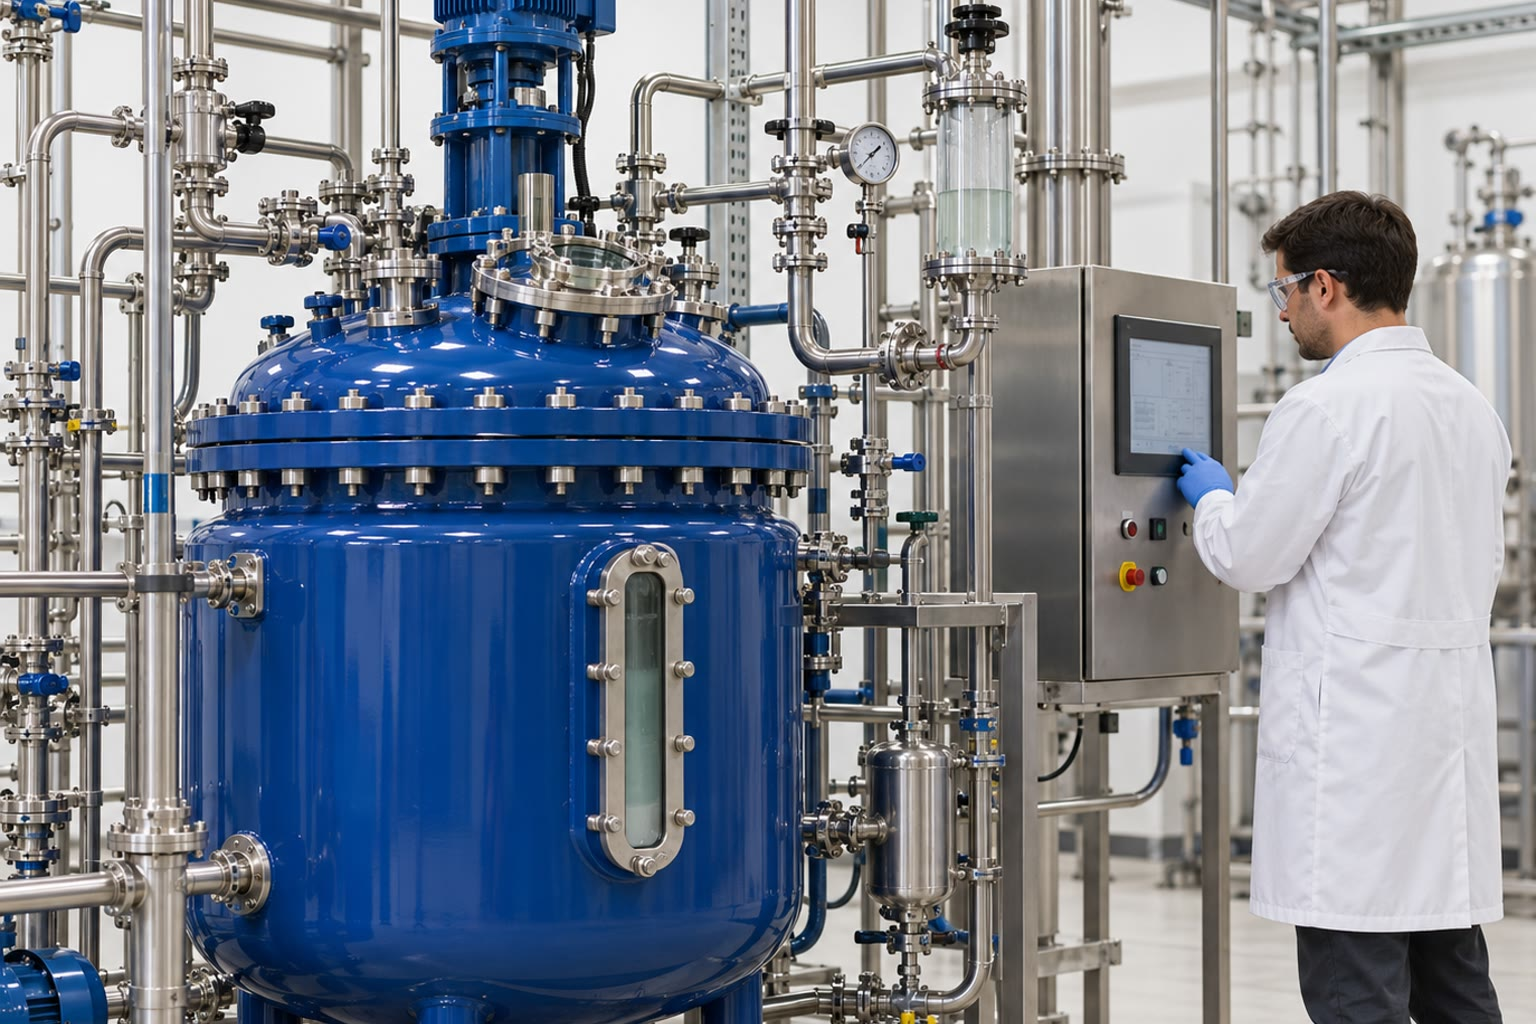
\includegraphics[width=0.62\linewidth]{images/book3/ai/b2-20-pilot-plant.jpg}

{\small A pilot plant of process chemistry: a glass-lined steel reactor, where a
catalysed coupling is scaled up from the flask before production.}
\end{omfigure}

\section{The language of organometallic complexes}

Organometallic complexes are counted as in \cref{met:b2:coordination-complexes:electron-count},
with a few more ligands: a hydride \ce{H-} and an alkyl or aryl anion \ce{R-} give two
electrons each and count $-1$ in the oxidation state; \ce{CO}, phosphines \ce{PR3} and
$\eta^2$-alkenes give two electrons and count 0; a halide \ce{X-} gives two and counts
$-1$.

\begin{definition}[Unsaturated complexes]\label{def:b2:catalytic-cycles:unsaturated}
A \emph{coordinatively unsaturated complex}\index{coordinatively unsaturated complex}
has fewer than 18 valence electrons (often 16) and can bind another ligand: it has a
\emph{vacant site}\index{vacant site}, a position of its \omterm{def:b2:coordination-complexes:coordination-sphere}{coordination sphere} free to
receive a two-electron donor.
\end{definition}

Square-planar $d^8$ complexes of rhodium(I), iridium(I), palladium(II) and
platinum(II) are 16-electron complexes; palladium(0) bisphosphines \ce{PdL2} have 14.
Such complexes are the active species of most \omterm{def:b2:catalytic-cycles:cycle}{catalytic cycles}.

\begin{method}[Counting an organometallic complex]\label{met:b2:catalytic-cycles:count-organometallic}
\begin{enumerate}
  \item List the ligands: anionic (\ce{H-}, \ce{R-}, \ce{X-}, \ce{C5H5-}) and neutral
        (\ce{CO}, \ce{PR3}, alkenes, solvent).
  \item Oxidation state = charge of the complex $-$ sum of the anionic ligand charges.
  \item $n = g -$ oxidation state; count = $n + 2 \times$(number of two-electron donors)
        $+$ 6 per $\eta^5$-\ce{C5H5-}.
  \item Coordination number = number of ligand positions occupied.
\end{enumerate}
\end{method}

\section{Ligand exchange, oxidative addition, reductive elimination}

\begin{definition}[Ligand exchange]\label{def:b2:catalytic-cycles:ligand-exchange}
A \emph{ligand exchange}\index{ligand exchange} is an elementary step in which a ligand of
the \omterm{def:b2:coordination-complexes:coordination-sphere}{coordination sphere} is replaced by another; it changes neither the oxidation state
nor, overall, the electron count. Its mechanisms are studied in the Year 3 volume.
\end{definition}

\begin{definition}[Oxidative addition and reductive elimination]\label{def:b2:catalytic-cycles:oxidative-addition}
In an \emph{oxidative addition}\index{oxidative addition}, a molecule A--B adds to a
metal centre by breaking its A--B bond and forming M--A and M--B bonds. A
\emph{reductive elimination}\index{reductive elimination} is the reverse step: two
ligands A and B, cis to each other, join into A--B and leave the metal.
\end{definition}

\begin{proposition}[Counting an oxidative addition]\label{prop:b2:catalytic-cycles:oa}
An \omterm{def:b2:catalytic-cycles:oxidative-addition}{oxidative addition} raises the oxidation state of the metal by 2, its \omterm{def:b2:coordination-complexes:electron-count}{valence electron
count} by 2 and its coordination number by 2; a \omterm{def:b2:catalytic-cycles:oxidative-addition}{reductive elimination} lowers each by 2.
\end{proposition}

\begin{proof}
A and B are counted as anions (\ce{H-}, \ce{R-}, \ce{X-}) once bound: two new anionic
ligands raise the oxidation state by 2 and lower $n$ by 2; they give two pairs, $+4$
electrons; the count changes by $-2 + 4 = +2$. Two positions are newly occupied. The
reverse step reverses every change.
\end{proof}

\begin{example}[Vaska's complex]\label{ex:b2:catalytic-cycles:vaska}
\ce{[IrCl(CO)(PPh3)2]}, square planar: iridium(I), $d^8$, 16 electrons, four-coordinate.
It adds dihydrogen: \ce{[IrH2Cl(CO)(PPh3)2]}, iridium(III), $d^6$, 18 electrons, octahedral,
the two hydrides cis.
\end{example}

\section{Insertion, elimination, transmetalation}

\begin{definition}[Insertion and $\beta$-hydride elimination]\label{def:b2:catalytic-cycles:insertion}
In a \emph{migratory insertion}\index{migratory insertion}, an unsaturated ligand
(alkene, \ce{CO}) bound to the metal inserts into a cis M--H or M--C bond: \ce{M-H} and an
alkene give an alkyl \ce{M-CH2-CH2-H}; \ce{M-R} and \ce{CO} give an acyl \ce{M-C(=O)R}.
A \emph{$\beta$-hydride elimination}\index{beta-hydride elimination@$\beta$-hydride
elimination} is the reverse of an alkene insertion: a hydrogen on the carbon $\beta$ to the
metal moves onto the metal, releasing an alkene.
\end{definition}

\begin{proposition}[Counting an insertion]\label{prop:b2:catalytic-cycles:insertion}
A \omterm{def:b2:catalytic-cycles:insertion}{migratory insertion} keeps the oxidation state and lowers the electron count by 2
(one ligand position is freed); a $\beta$-hydride elimination raises the count by 2.
\end{proposition}

\begin{proof}
Before: \ce{H-} (or \ce{R-}, anionic) and the alkene (neutral), two ligands, four electrons.
After: one alkyl (anionic), two electrons. The anionic charge is unchanged: same
oxidation state; two electrons and one position lost.
\end{proof}

\begin{proposition}[Conditions for $\beta$-hydride elimination]\label{prop:b2:catalytic-cycles:beta-h}
A metal alkyl undergoes $\beta$-hydride elimination only if the alkyl carries a hydrogen on
its $\beta$ carbon and the metal has a \omterm{def:b2:catalytic-cycles:unsaturated}{vacant site} cis to the alkyl.
\end{proposition}

\begin{proof}[Argument]
The step goes through a four-membered arrangement M--C$_\alpha$--C$_\beta$--H in which the
hydrogen reaches the metal: it needs that hydrogen, and an empty position next to the alkyl
to receive it. Methyl, benzyl, neopentyl and aryl groups, which have no $\beta$ hydrogen
able to reach the metal, are stable towards it.
\end{proof}

\begin{definition}[Transmetalation]\label{def:b2:catalytic-cycles:transmetalation}
A \emph{transmetalation}\index{transmetalation} transfers an organic group from one metal
(or metalloid: boron, zinc, tin) to another, usually in exchange for a halide.
\end{definition}

\begin{omfigure}
\begin{tikzpicture}[font=\small, >={Stealth}]
  \tikzset{omstepar/.style={->, thick}}
  \foreach \y/\l/\r/\top/\bot/\rev in {
      0/{$\mathrm{L}_n\mathrm{M}$}/{$\mathrm{L}_n\mathrm{M(A)(B)}$}/{+ A--B}/{oxidative addition}/{reductive elimination},
      -1.5/{$\mathrm{L}_n\mathrm{M(H)(CH_2{=}CH_2)}$}/{$\mathrm{L}_n\mathrm{M{-}CH_2CH_3}$}/{}/{migratory insertion}/{$\beta$-hydride elimination},
      -3.0/{$\mathrm{L}_n\mathrm{M(X)(R)}$}/{$\mathrm{L}_n\mathrm{M(R)(R')}$}/{+ R$'$--[B], $-$ X--[B]}/{transmetalation}/{},
      -4.5/{$\mathrm{L}_n\mathrm{M(X)}$}/{$\mathrm{L}_n\mathrm{M(X)(L')}$}/{+ L$'$}/{ligand exchange or binding}/{}} {
    \node[cyclenode, anchor=east] (l) at (0,\y) {\l};
    \node[cyclenode, anchor=west] (r) at (5.2,\y) {\r};
    \draw[omstepar] ($(l.east)+(0.1,0.08)$) -- ($(r.west)+(-0.1,0.08)$) node[midway, above, font=\scriptsize] {\top};
    \node[font=\scriptsize, anchor=north] at (2.6,\y-0.02) {\bot};
    \node[font=\scriptsize, black!55, anchor=west] at (5.2,\y-0.5) {\rev};
  }
\end{tikzpicture}

{\small The elementary steps of organometallic catalysis. \omterm{def:b2:catalytic-cycles:oxidative-addition}{Oxidative addition}: oxidation
state, count and coordination number $+2$; \omterm{def:b2:catalytic-cycles:oxidative-addition}{reductive elimination}: $-2$. \omterm{def:b2:catalytic-cycles:insertion}{Migratory
insertion}: count $-2$, oxidation state unchanged; $\beta$-hydride elimination: the
reverse. \omterm{def:b2:catalytic-cycles:transmetalation}{Transmetalation}: an organic group moves to the metal from boron, zinc or tin.}
\end{omfigure}

\section{Reading a catalytic cycle}

\begin{definition}[Catalytic cycle]\label{def:b2:catalytic-cycles:cycle}
A \emph{catalytic cycle}\index{catalytic cycle} is a closed sequence of elementary steps
that consumes the reagents, releases the products and regenerates its first complex. The
compound added to the reaction, which turns into the first complex of the cycle, is the
\emph{precatalyst}\index{precatalyst}. The \emph{turnover number}\index{turnover number}
(TON) is the amount of product formed per amount of catalyst; the \emph{turnover
frequency}\index{turnover frequency} (TOF) is the turnover number per unit time.
\end{definition}

\begin{proposition}[The overall equation]\label{prop:b2:catalytic-cycles:cycle-sum}
The sum of the steps of a \omterm{def:b2:catalytic-cycles:cycle}{catalytic cycle} is the equation of the catalysed reaction:
every metal complex appears once as a product and once as a reactant, and cancels.
\end{proposition}

\begin{proof}
The cycle being closed, each intermediate is formed by one step and consumed by the next;
adding the steps, these species appear on both sides and cancel. What remains are the
species that enter from outside (reagents) and leave (products).
\end{proof}

\begin{method}[Reading a cycle]\label{met:b2:catalytic-cycles:read-cycle}
\begin{enumerate}
  \item For each complex, compute the oxidation state, the electron count and the
        coordination number.
  \item Name each step from the changes ($+2/+2/+2$: \omterm{def:b2:catalytic-cycles:oxidative-addition}{oxidative addition}; count $-2$ at
        constant oxidation state: insertion; and so on).
  \item Check that no complex exceeds 18 electrons and that a step needing a \omterm{def:b2:catalytic-cycles:unsaturated}{vacant site}
        starts from an unsaturated complex.
  \item Add the steps: the sum must be the overall equation.
\end{enumerate}
\end{method}

\begin{omfigure}
\begin{tikzpicture}[font=\small, >={Stealth}]
  \node[cyclenode] (n1) at (90:2.3) {\ce{[RhCl(PPh3)2]}\\ Rh(I), 14 e};
  \node[cyclenode] (n2) at (0:3.4) {\ce{[RhH2Cl(PPh3)2]}\\ Rh(III), 16 e};
  \node[cyclenode] (n3) at (270:2.3) {\ce{[RhH2Cl(PPh3)2(alkene)]}\\ Rh(III), 18 e};
  \node[cyclenode] (n4) at (180:3.4) {\ce{[RhH(alkyl)Cl(PPh3)2]}\\ Rh(III), 16 e};
  \draw[cyclearc] (n1) to[bend left=20] node[cyclelabel, below left] {oxidative\\ addition} (n2);
  \draw[cyclearc] (n2) to[bend left=20] node[cyclelabel, left=12pt] {alkene\\ binding} (n3);
  \draw[cyclearc] (n3) to[bend left=20] node[cyclelabel, above right] {migratory\\ insertion} (n4);
  \draw[cyclearc] (n4) to[bend left=20] node[cyclelabel, below right] {reductive\\ elimination} (n1);
  \draw[cyclein] (4.6,2.3) node[right] {\ce{H2}} -- (2.6,1.75);
  \draw[cyclein] (4.6,-2.3) node[right] {alkene} -- (2.6,-1.75);
  \draw[cycleout] (-2.6,1.75) -- (-4.6,2.3) node[left] {alkane};
  \node[font=\scriptsize, align=center, black!60] at (0,-0.05) {precatalyst\\ \ce{[RhCl(PPh3)3]}\\ loses one \ce{PPh3}};
\end{tikzpicture}

{\small The hydrogenation of an alkene with Wilkinson's catalyst, simplified (phosphine
and solvent exchanges omitted). The four steps sum to $\ce{alkene + H2 -> alkane}$; the
rhodium complexes cancel.}
\end{omfigure}

\begin{omfigure}
\begin{tikzpicture}[font=\small, >={Stealth}]
  \node[cyclenode] (s1) at (90:2.3) {\ce{PdL2}\\ Pd(0), 14 e};
  \node[cyclenode] (s2) at (0:3.4) {\ce{[ArPd(Br)L2]}\\ Pd(II), 16 e};
  \node[cyclenode] (s3) at (270:2.3) {$[\mathrm{ArPd(Ar')L_2}]$\\ Pd(II), 16 e};
  \draw[cyclearc] (s1) to[bend left=25] node[cyclelabel, below left] {oxidative\\ addition} (s2);
  \draw[cyclearc] (s2) to[bend left=25] node[cyclelabel, above left] {transmetalation} (s3);
  \draw[cyclearc] (s3) to[bend left=35] node[cyclelabel, right] {reductive\\ elimination} (s1);
  \draw[cyclein] (4.8,2.2) node[right] {\ce{Ar-Br}} -- (2.6,1.6);
  \draw[cyclein] (5.4,-0.9) node[right, align=left] {$\mathrm{Ar'B(OH)_2}$\\ + base} -- (3.3,-1.2);
  \draw[cycleout] (2.3,-2.0) -- (4.4,-2.9) node[right] {\ce{Br-}, \ce{B(OH)3}};
  \draw[cycleout] (-1.75,-0.4) -- (-4.2,-0.4) node[left] {$\mathrm{Ar{-}Ar'}$};
\end{tikzpicture}

{\small The Suzuki coupling, simplified. Palladium(0) adds the aryl bromide; the base
turns the boronic acid into a borate, which transfers its aryl group to palladium; the two
aryls, cis, are eliminated as the biaryl, regenerating palladium(0).}
\end{omfigure}

In the Heck reaction, the aryl--palladium complex formed by \omterm{def:b2:catalytic-cycles:oxidative-addition}{oxidative addition} binds an
alkene instead of a borate; \omterm{def:b2:catalytic-cycles:insertion}{migratory insertion} puts the aryl on the alkene, and a
$\beta$-hydride elimination releases the substituted alkene (usually the trans isomer)
and a palladium hydride, from which a base removes \ce{HBr} to regenerate palladium(0).

Hydroformylation, the addition of \ce{H2} and \ce{CO} across an alkene to give an aldehyde,
runs on cobalt or rhodium hydrides through insertion of the alkene, insertion of \ce{CO}
into the metal--alkyl bond, \omterm{def:b2:catalytic-cycles:oxidative-addition}{oxidative addition} of \ce{H2} and \omterm{def:b2:catalytic-cycles:oxidative-addition}{reductive elimination} of the
aldehyde. The direction of the first insertion decides the product: the metal on the
terminal carbon gives the linear aldehyde, on the inner carbon the branched one; bulky
phosphines favour the linear product.

\begin{history}[Cross-coupling]
\begin{minipage}[t]{0.36\linewidth}
\vspace{0pt}
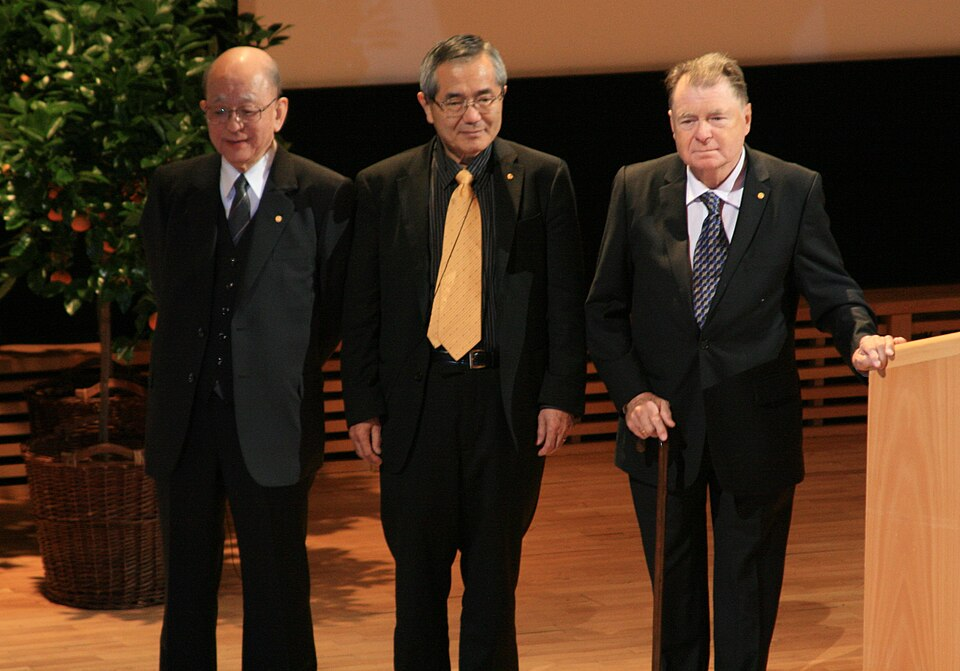
\includegraphics[width=\linewidth]{images/book3/nobel-2010.jpg}
\end{minipage}\hfill
\begin{minipage}[t]{0.6\linewidth}
\vspace{0pt}
Palladium-catalysed couplings of aryl and vinyl halides with alkenes (Richard Heck, from
1968), with organozinc reagents (Ei-ichi Negishi, 1977) and with organoboron compounds
(Akira Suzuki, 1979) made the joining of two carbon frameworks routine; they are now among
the most used reactions in the making of medicines and materials. The Nobel Prize in
Chemistry was awarded to the three in 2010. (Photograph: Suzuki, Negishi and Heck, left
to right, 2010; BloodIce, CC BY-SA 4.0, Wikimedia Commons.)
\end{minipage}
\end{history}

\begin{proposition}[Turnover]\label{prop:b2:catalytic-cycles:tof}
With $n_P$ the amount of product formed in a time $t$ by an amount $n_{\text{cat}}$ of catalyst,
$\mathrm{TON} = n_P/n_{\text{cat}}$ and the mean \omterm{def:b2:catalytic-cycles:cycle}{turnover frequency} is $\mathrm{TOF} =
\mathrm{TON}/t$.
\end{proposition}

\begin{proof}
Each turn of the cycle makes one product molecule per metal atom; the number of turns made
by each atom on average is $n_P/n_{\text{cat}}$, and the rate of turning is that number per unit
time.
\end{proof}

\begin{safety}{\ghs[5mm]{GHS05}\,\ghs[5mm]{GHS07}\,\ghs[5mm]{GHS09}}
Palladium(II) ethanoate is corrosive to the eyes and toxic to aquatic life;
triphenylphosphine is harmful and a sensitiser. They are weighed in a fume hood, and the
palladium residues are collected for recovery, never poured down the drain.
% ledger: ghs:Pd-acetate, ghs:PPh3, ghs:phenylboronic-acid, ghs:4-bromotoluene
\end{safety}

\section{Exercises}

\begin{exercise}[$\star$]\label{exo:b2:catalytic-cycles:1}
Give the oxidation state, $d^n$ and electron count of Vaska's complex
\ce{[IrCl(CO)(PPh3)2]} before and after it adds \ce{H2}.
\end{exercise}

\begin{exercise}[$\star$]\label{exo:b2:catalytic-cycles:2}
Name the step: \ce{[PtCl2(CH3)2(PR3)2] -> [PtCl2(PR3)2] + C2H6}; \ce{[Pd(Ph)Br(PR3)2] +
CH2=CH2 -> [Pd(CH2CH2Ph)Br(PR3)] + PR3}.
\end{exercise}

\begin{exercise}[$\star$]\label{exo:b2:catalytic-cycles:3}
A reaction uses \qty{0.020}{mmol} of catalyst and gives \qty{15.0}{mmol} of product in
\qty{3.0}{h}. Compute the TON and the mean TOF.
\end{exercise}

\begin{exercise}[$\star$]\label{exo:b2:catalytic-cycles:4}
Add the three steps of the Suzuki cycle and check that palladium cancels.
\end{exercise}

\begin{exercise}[$\star\star$]\label{exo:b2:catalytic-cycles:5}
Which of these alkyl palladium complexes can undergo $\beta$-hydride elimination:
\ce{Pd-CH3}, \ce{Pd-CH2CH3}, \ce{Pd-CH2C(CH3)3}, \ce{Pd-CH2Ph}, \ce{Pd-CH(CH3)2}?
\end{exercise}

\begin{exercise}[$\star\star$]\label{exo:b2:catalytic-cycles:6}
Predict the product of the Heck reaction of iodobenzene with methyl propenoate, and its
geometry.
\end{exercise}

\begin{exercise}[$\star\star$]\label{exo:b2:catalytic-cycles:7}
Write the linear and branched aldehydes formed by the hydroformylation of propene, and
explain which insertion leads to each.
\end{exercise}

\begin{exercise}[$\star\star$]\label{exo:b2:catalytic-cycles:8}
Why can \ce{[RhCl(PPh3)3]} add \ce{H2} only after losing a phosphine, while
\ce{[RhCl(PPh3)2]} adds it at once?
\end{exercise}

\begin{exercise}[$\star\star$]\label{exo:b2:catalytic-cycles:9}
In the Suzuki coupling, why is a base needed, and what does it do to the boronic acid?
\end{exercise}

\begin{exercise}[$\star\star\star$]\label{exo:b2:catalytic-cycles:10}
A proposed cycle for the hydrogenation of an alkene on a $d^8$ complex \ce{ML3X} (16 e)
starts with the binding of the alkene to give a 20-electron complex, then \omterm{def:b2:catalytic-cycles:oxidative-addition}{oxidative addition}
of \ce{H2}. Find the error and correct the order.
\end{exercise}

\begin{exercise}[$\star\star\star$]\label{exo:b2:catalytic-cycles:11}
The amount of product of a catalysed reaction grows as $n_P(t) = n_{\max}(1 - \mathrm e^{-t/\tau})$
with $n_{\max} = \qty{10.0}{mmol}$, $\tau = \qty{40}{min}$ and \qty{0.010}{mmol} of catalyst
(exercise data). Compute the initial TOF and the final TON.
\end{exercise}

\begin{exercise}[$\star\star\star$]\label{exo:b2:catalytic-cycles:12}
Propose a cross-coupling to prepare 4-methoxybiphenyl, choosing the halide and the boronic
acid, and write the cycle.
\end{exercise}

\section{Problem: Reading the Suzuki Cycle}

\begin{problem}[{Weekend problem --- the precatalyst and the active palladium(0), the
oxidative addition, transmetalation and reductive elimination of a Suzuki coupling, the
yield and the turnover number, and the side reactions}]
\label{pb:b2:catalytic-cycles:1}
Run (exercise data): \qty{10.0}{mmol} of 4-bromotoluene, \qty{12.0}{mmol} of
phenylboronic acid, \qty{20}{mmol} of potassium carbonate, \qty{0.050}{mmol} of palladium(II)
ethanoate and \qty{0.10}{mmol} of triphenylphosphine in a mixture of toluene, ethanol and
water, heated under nitrogen; isolated product: \qty{1.51}{g} of 4-methylbiphenyl. Molar
masses (\unit{g/mol}): 4-bromotoluene 171.04, phenylboronic acid 121.93, 4-methylbiphenyl
168.24, palladium(II) ethanoate 224.51.
% ledger: aw:C, aw:H, aw:Br, aw:B, aw:O, aw:Pd

\medskip
\noindent\textbf{Part I --- The catalyst.}
\begin{enumerate}
  \item Give the oxidation state and $d^n$ of palladium in palladium(II) ethanoate.
  \item In the flask it is reduced to \ce{Pd(PPh3)2}. Give its oxidation state, $d^n$ and
        electron count.
  \item Why is that complex coordinatively unsaturated?
  \item Why is the reaction run under nitrogen?
  \item What is the role of the excess triphenylphosphine?
  \item Is palladium(II) ethanoate the catalyst or the \omterm{def:b2:catalytic-cycles:cycle}{precatalyst}?
\end{enumerate}

\medskip
\noindent\textbf{Part II --- The steps.}
\begin{enumerate}[resume]
  \item Write the \omterm{def:b2:catalytic-cycles:oxidative-addition}{oxidative addition} of 4-bromotoluene and count the product.
  \item What does the carbonate do to phenylboronic acid?
  \item Write the \omterm{def:b2:catalytic-cycles:transmetalation}{transmetalation}.
  \item Why must the two aryl groups be cis before the next step?
  \item Write the \omterm{def:b2:catalytic-cycles:oxidative-addition}{reductive elimination} and count the palladium species formed.
  \item Add the three steps.
\end{enumerate}

\medskip
\noindent\textbf{Part III --- Yield and turnover.}
\begin{enumerate}[resume]
  \item Which reagent is limiting?
  \item Compute the amount of product isolated.
  \item Compute the yield.
  \item Compute the catalyst loading in mol~\% relative to the bromide.
  \item Compute the \omterm{def:b2:catalytic-cycles:cycle}{turnover number} of palladium.
  \item The run took \qty{4.0}{h}. Compute the mean \omterm{def:b2:catalytic-cycles:cycle}{turnover frequency} per hour.
\end{enumerate}

\medskip
\noindent\textbf{Part IV --- Side reactions.}
\begin{enumerate}[resume]
  \item Some biphenyl \ce{Ph-Ph} is found. Suggest how it forms.
  \item Why is no $\beta$-hydride elimination possible here?
  \item An aryl chloride reacts much more slowly than the bromide. Which step suffers?
  \item What happens to the palladium at the end of the reaction, and why is it recovered?
  \item Why is a small excess of boronic acid used?
  \item State the \omterm{def:b2:catalytic-cycles:cycle}{turnover number} of palladium in the run.
\end{enumerate}
\end{problem}
